\section{Matching Problem}
    \subsection{Provide mathematical formulation of a matching problem}
    Given a graph 
    \begin{align}
        G\left(V,E\right) \quad &\text{where:} \\
        & V = \text{set of nodes (i.e. set of numbers)}\\
        & E = \{\{x,y\} \;|\; x,y \in V \wedge x \neq y  \}\\
         &\text{a matching is a set defined as:}\\
       &M = \{e_1 \in E | \forall e_2 in E \wedge e_1 = e_2 
            \Rightarrow  \{e_{1_x}, e_{1_y}\} \cap \{e_{2_x}, e_{2_y}\} = \emptyset\}
    \end{align}
    In words: a matching is a subset of edges that don't have any node in common. 
    A matching problem is the problem of finding the best matching given a graph. 


    \subsection{Describe what alternating and augmenti paths are}
        W.r.t. the above definitions we have that 
        \begin{itemize}
            \item An alternating path is a path inside the graph composed by edges that are in M and edges that are not.
            \item An augmenting path is an alternating path where the first and the last node are not in the matching set 
        \end{itemize}

    \subsection{Describe the functioning of the alternating-path algorithms for bipartite graphs}
    In bipartite graphs alternating-path algorithms aim to find best solutions to matching problems. They rely on finding an augmenting path that later is converted into a matching of higher cardinality of the one given.

    \subsection{Describe the functioning of the alternating-path algorithms for arbitrary graphs}
    Same as previous?



    \section{Alternating-path algorithms for bipartite graphs}
    \subsection{Given a bipartite graph and a matching, apply alternating-path algorithm to find all shortes augmenting paths, if any}
    Given the graph below we want to expand all the unmatched nodes in order to find a beter matching. We aim to find shortest augmenting paths so we'll apply $BFS$ to expand nodes in the following way:
    \begin{itemize}
        \item starting from one unmatched node we expand it through its unexpanded edges
            \subitem - if expand following the alternating policy (if we find a matched node
            we follow expand also through the match edge). We mark the final node as even
            \subitem - if we find a non mathced node we stop and we add it to the nodes to be expanded (should we mark it as even?)
        \item we mark that node as expanded 
        \item we continue the expanding procedure
        \item if we find an even node of another subtree we found an augmen path and we can improve the matching
        \item if we find an odd node we can stop the search (nothing happens)
    \end{itemize}


    \section{Alternating-path algorithms for arbitrary graphs}
    \subsection{Given a arbitrary graph and a matching, apply alternating-path algorithm to find all shortes augmenting paths, if any}
    The procedure is the same as bipartite but we have the additional case in which we could fall into node of the same subgraph: in this case we found a blossom. At this point we can collapse the blossom and consider it as a single node and then continue the search. At the end we'll expand again the blossom and we'll have found an augmenting path if we've found it with collapsed blossom. In other words the blossom does not affect the search of augmen paths. 

    \section{Combinatorial bandits}
    \subsection{Define what a combinatorial bandit problem is.}
    A combinatorial bandit problem is a problem where arms are correlated each other and we can pull more then one arm per turn, called super arm, and arms are regolated by a combinatorial constraint (i.e. knapsack, Independend set, matching)
    \subsection{Describe how a matching problem can be formulates as a combinatorial bandit problem}
    A matching problem can be seen as CMAB where arms are the nodes of a given graphs and a superarm is a matching. We wanto to maximize the matching but keeping the constraint about the matching policies. 

    \subsection{Describe the Combinatorial Thompson Sampling algorithm.}
    In CTS we have distributions over nodes. Each round we sample the nodes to compose a super arm. We apply an optimizer to make the combinatorial problem be maximized/respected. 
    Then we play the arm and update the distributions. 

    \subsection{Define the regret in the case of combinatorial bandit problem and discuss the differences between the  regret bounds of the non-combinatorial and combinatorial cases.}
    (How the hell is calculated the regret?)\\
    Standard regret bound is
    \begin{equation}
        R_T \leq O \left( \sum_{a_i in A, \; a_i \neq a^*} \dfrac{\Lambda_i}{KL(R(a_i), R(a_*)) } \cdot \left(\log T + \log \log T\right) \right)
    \end{equation}
    In the CMAB instead we have:
    \begin{equation}
        R_T \leq O \left( |A| \dfrac{\log T}{\Lambda_{min}} \right)
    \end{equation}
    If we use non exact optimization algorithm the regret increases
    

    \section{Online Matching}
    \subsection{Define what an online matching problem is and how it distinguishes from the non-online case}
    An online matching problem is a matching problem that is not fully observable. In particular we can observe only a subset of nodes at each time step $t$.

    \subsection{Define the competitive factor of an online problem.}
    The competitive factor is defined as: 
    \begin{equation}
        C = min_{P}\dfrac{\Gamma(P)}{\Gamma_{calirvoyant}(P)}
    \end{equation}

    \subsection{Show that a basic online matching problem (in bipartite graphs, with the nodes of only side entering dynamically) does not admit any deterministic algorithm with competitive factor larger than 1/2.}
    We can see in the following image that can't be greater then 1/2
    

\tikzset{every picture/.style={line width=0.75pt}} %set default line width to 0.75pt        

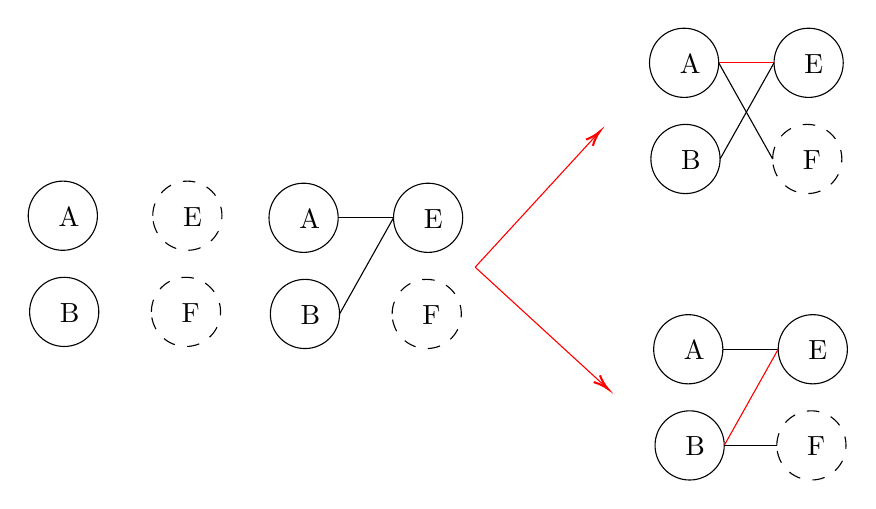
\begin{tikzpicture}[x=0.5pt,y=0.5pt,yscale=-1,xscale=1]
%uncomment if require: \path (0,480); %set diagram left start at 0, and has height of 480

%Shape: Circle [id:dp9661643343228774] 
\draw   (27,168) .. controls (27,154.19) and (38.19,143) .. (52,143) .. controls (65.81,143) and (77,154.19) .. (77,168) .. controls (77,181.81) and (65.81,193) .. (52,193) .. controls (38.19,193) and (27,181.81) .. (27,168) -- cycle ;
%Shape: Circle [id:dp12560412512444952] 
\draw  [dash pattern={on 4.5pt off 4.5pt}] (117,168) .. controls (117,154.19) and (128.19,143) .. (142,143) .. controls (155.81,143) and (167,154.19) .. (167,168) .. controls (167,181.81) and (155.81,193) .. (142,193) .. controls (128.19,193) and (117,181.81) .. (117,168) -- cycle ;
%Shape: Circle [id:dp16800153090175107] 
\draw   (28,237.5) .. controls (28,223.69) and (39.19,212.5) .. (53,212.5) .. controls (66.81,212.5) and (78,223.69) .. (78,237.5) .. controls (78,251.31) and (66.81,262.5) .. (53,262.5) .. controls (39.19,262.5) and (28,251.31) .. (28,237.5) -- cycle ;
%Shape: Circle [id:dp02567101163702956] 
\draw  [dash pattern={on 4.5pt off 4.5pt}] (116,237.5) .. controls (116,223.69) and (127.19,212.5) .. (141,212.5) .. controls (154.81,212.5) and (166,223.69) .. (166,237.5) .. controls (166,251.31) and (154.81,262.5) .. (141,262.5) .. controls (127.19,262.5) and (116,251.31) .. (116,237.5) -- cycle ;
%Shape: Circle [id:dp704872757667049] 
\draw   (201,169.5) .. controls (201,155.69) and (212.19,144.5) .. (226,144.5) .. controls (239.81,144.5) and (251,155.69) .. (251,169.5) .. controls (251,183.31) and (239.81,194.5) .. (226,194.5) .. controls (212.19,194.5) and (201,183.31) .. (201,169.5) -- cycle ;
%Shape: Circle [id:dp9541917502607109] 
\draw   (291,169.5) .. controls (291,155.69) and (302.19,144.5) .. (316,144.5) .. controls (329.81,144.5) and (341,155.69) .. (341,169.5) .. controls (341,183.31) and (329.81,194.5) .. (316,194.5) .. controls (302.19,194.5) and (291,183.31) .. (291,169.5) -- cycle ;
%Shape: Circle [id:dp9834500234358272] 
\draw   (202,239) .. controls (202,225.19) and (213.19,214) .. (227,214) .. controls (240.81,214) and (252,225.19) .. (252,239) .. controls (252,252.81) and (240.81,264) .. (227,264) .. controls (213.19,264) and (202,252.81) .. (202,239) -- cycle ;
%Shape: Circle [id:dp745177232320891] 
\draw  [dash pattern={on 4.5pt off 4.5pt}] (290,239) .. controls (290,225.19) and (301.19,214) .. (315,214) .. controls (328.81,214) and (340,225.19) .. (340,239) .. controls (340,252.81) and (328.81,264) .. (315,264) .. controls (301.19,264) and (290,252.81) .. (290,239) -- cycle ;
%Straight Lines [id:da6373671172965589] 
\draw    (251,169.5) -- (291,169.5) ;
%Straight Lines [id:da37705224633079504] 
\draw    (252,239) -- (291,169.5) ;
%Straight Lines [id:da188038606373649] 
\draw [color={rgb, 255:red, 255; green, 0; blue, 0 }  ,draw opacity=1 ]   (350,205.19) -- (438.65,108.66) ;
\draw [shift={(440,107.19)}, rotate = 132.56] [color={rgb, 255:red, 255; green, 0; blue, 0 }  ,draw opacity=1 ][line width=0.75]    (10.93,-3.29) .. controls (6.95,-1.4) and (3.31,-0.3) .. (0,0) .. controls (3.31,0.3) and (6.95,1.4) .. (10.93,3.29)   ;
%Straight Lines [id:da9644672372423333] 
\draw [color={rgb, 255:red, 255; green, 0; blue, 0 }  ,draw opacity=1 ]   (350,205.19) -- (444.53,291.84) ;
\draw [shift={(446,293.19)}, rotate = 222.51] [color={rgb, 255:red, 255; green, 0; blue, 0 }  ,draw opacity=1 ][line width=0.75]    (10.93,-3.29) .. controls (6.95,-1.4) and (3.31,-0.3) .. (0,0) .. controls (3.31,0.3) and (6.95,1.4) .. (10.93,3.29)   ;
%Shape: Circle [id:dp07385836151839431] 
\draw   (476,57.5) .. controls (476,43.69) and (487.19,32.5) .. (501,32.5) .. controls (514.81,32.5) and (526,43.69) .. (526,57.5) .. controls (526,71.31) and (514.81,82.5) .. (501,82.5) .. controls (487.19,82.5) and (476,71.31) .. (476,57.5) -- cycle ;
%Shape: Circle [id:dp9165583980924612] 
\draw   (566,57.5) .. controls (566,43.69) and (577.19,32.5) .. (591,32.5) .. controls (604.81,32.5) and (616,43.69) .. (616,57.5) .. controls (616,71.31) and (604.81,82.5) .. (591,82.5) .. controls (577.19,82.5) and (566,71.31) .. (566,57.5) -- cycle ;
%Shape: Circle [id:dp6912511925881482] 
\draw   (477,127) .. controls (477,113.19) and (488.19,102) .. (502,102) .. controls (515.81,102) and (527,113.19) .. (527,127) .. controls (527,140.81) and (515.81,152) .. (502,152) .. controls (488.19,152) and (477,140.81) .. (477,127) -- cycle ;
%Shape: Circle [id:dp3744250561798852] 
\draw  [dash pattern={on 4.5pt off 4.5pt}] (565,127) .. controls (565,113.19) and (576.19,102) .. (590,102) .. controls (603.81,102) and (615,113.19) .. (615,127) .. controls (615,140.81) and (603.81,152) .. (590,152) .. controls (576.19,152) and (565,140.81) .. (565,127) -- cycle ;
%Straight Lines [id:da31957420654440494] 
\draw [color={rgb, 255:red, 255; green, 0; blue, 0 }  ,draw opacity=1 ]   (526,57.5) -- (566,57.5) ;
%Straight Lines [id:da020346885140927418] 
\draw    (527,127) -- (566,57.5) ;
%Shape: Circle [id:dp9237954684244705] 
\draw   (479,264.5) .. controls (479,250.69) and (490.19,239.5) .. (504,239.5) .. controls (517.81,239.5) and (529,250.69) .. (529,264.5) .. controls (529,278.31) and (517.81,289.5) .. (504,289.5) .. controls (490.19,289.5) and (479,278.31) .. (479,264.5) -- cycle ;
%Shape: Circle [id:dp2095586363473656] 
\draw   (569,264.5) .. controls (569,250.69) and (580.19,239.5) .. (594,239.5) .. controls (607.81,239.5) and (619,250.69) .. (619,264.5) .. controls (619,278.31) and (607.81,289.5) .. (594,289.5) .. controls (580.19,289.5) and (569,278.31) .. (569,264.5) -- cycle ;
%Shape: Circle [id:dp2874395327193138] 
\draw   (480,334) .. controls (480,320.19) and (491.19,309) .. (505,309) .. controls (518.81,309) and (530,320.19) .. (530,334) .. controls (530,347.81) and (518.81,359) .. (505,359) .. controls (491.19,359) and (480,347.81) .. (480,334) -- cycle ;
%Shape: Circle [id:dp7304682465324399] 
\draw  [dash pattern={on 4.5pt off 4.5pt}] (568,334) .. controls (568,320.19) and (579.19,309) .. (593,309) .. controls (606.81,309) and (618,320.19) .. (618,334) .. controls (618,347.81) and (606.81,359) .. (593,359) .. controls (579.19,359) and (568,347.81) .. (568,334) -- cycle ;
%Straight Lines [id:da4711403306401545] 
\draw    (529,264.5) -- (569,264.5) ;
%Straight Lines [id:da826424249425568] 
\draw [color={rgb, 255:red, 255; green, 0; blue, 0 }  ,draw opacity=1 ]   (530,334) -- (569,264.5) ;
%Straight Lines [id:da5339917948126969] 
\draw    (526,57.5) -- (565,127) ;
%Straight Lines [id:da9215252260981803] 
\draw    (530,334) -- (568,334) ;

% Text Node
\draw (47,160) node [anchor=north west][inner sep=0.75pt]   [align=left] {A};
% Text Node
\draw (137,160) node [anchor=north west][inner sep=0.75pt]   [align=left] {E};
% Text Node
\draw (48,229.5) node [anchor=north west][inner sep=0.75pt]   [align=left] {B};
% Text Node
\draw (136,229.5) node [anchor=north west][inner sep=0.75pt]   [align=left] {F};
% Text Node
\draw (221,161.5) node [anchor=north west][inner sep=0.75pt]   [align=left] {A};
% Text Node
\draw (311,161.5) node [anchor=north west][inner sep=0.75pt]   [align=left] {E};
% Text Node
\draw (222,231) node [anchor=north west][inner sep=0.75pt]   [align=left] {B};
% Text Node
\draw (310,231) node [anchor=north west][inner sep=0.75pt]   [align=left] {F};
% Text Node
\draw (496,49.5) node [anchor=north west][inner sep=0.75pt]   [align=left] {A};
% Text Node
\draw (586,49.5) node [anchor=north west][inner sep=0.75pt]   [align=left] {E};
% Text Node
\draw (497,119) node [anchor=north west][inner sep=0.75pt]   [align=left] {B};
% Text Node
\draw (585,119) node [anchor=north west][inner sep=0.75pt]   [align=left] {F};
% Text Node
\draw (499,256.5) node [anchor=north west][inner sep=0.75pt]   [align=left] {A};
% Text Node
\draw (589,256.5) node [anchor=north west][inner sep=0.75pt]   [align=left] {E};
% Text Node
\draw (500,326) node [anchor=north west][inner sep=0.75pt]   [align=left] {B};
% Text Node
\draw (588,326) node [anchor=north west][inner sep=0.75pt]   [align=left] {F};


\end{tikzpicture}



    \subsection{Describe a greedy algorithm for a basic online matching problem with competitive factor 1 - 1/e}
    A greedy algorithm with $1-1/e$ is simply an algorithm that at each timestep matches unmached nodes with the first unmached node


    \section{General online matching}
    \subsection{Show that when both sides of a bipartite matching problem enter dynamically there is not online algorithm with strictly positive competitive factor}
    \input{Matching/images/1_6_1_no_positive_alg}

    \subsection{Describe the functioning of the Postponed Dynamic Deferred Acceptance and report an example.}
    I really do not understand this algorithm 